\documentclass[conference]{IEEEtran}
\IEEEoverridecommandlockouts

\usepackage{cite}
\usepackage{amsmath,amssymb,amsfonts}
\usepackage{graphicx}
\usepackage{textcomp}
\usepackage{xcolor}
\usepackage{algorithm}
\usepackage{algpseudocode}
\usepackage{multirow}
\usepackage{listings}
\usepackage{tabularray}


\definecolor{codegreen}{rgb}{0,0.6,0}
\definecolor{codegray}{rgb}{0.5,0.5,0.5}
\definecolor{codepurple}{rgb}{0.58,0,0.82}
\definecolor{backcolour}{rgb}{0.95,0.95,0.92}

\lstset{
    backgroundcolor=\color{backcolour},   
    commentstyle=\color{codegreen},
    keywordstyle=\color{magenta},
    numberstyle=\tiny\color{codegray},
    stringstyle=\color{codepurple},
    basicstyle=\footnotesize\ttfamily,
    breakatwhitespace=false,         
    breaklines=true,                 
    captionpos=b,                    
    keepspaces=true,                 
    numbers=left,                    
    numbersep=5pt,                  
    showspaces=false,                
    showstringspaces=false,
    showtabs=false,                  
    tabsize=2,
    language=C
}

\def\BibTeX{{\rm B\kern-.05em{\sc i\kern-.025em b}\kern-.08em
    T\kern-.1667em\lower.7ex\hbox{E}\kern-.125emX}}
\begin{document}

\title{COMP2432 Group Project: 
Steel-making Production Line Scheduler (PLS)}

\author{\IEEEauthorblockN{1\textsuperscript{st} Yuhang DAI}
\IEEEauthorblockA{\textit{Department of Computing} \\
\textit{The Hong Kong Polytechnic University}\\
Hong Kong SAR, China \\
22097845d@connect.polyu.hk}
\and
\IEEEauthorblockN{2\textsuperscript{nd} Zhanzhi LIN}
\IEEEauthorblockA{\textit{Department of Computing} \\
\textit{The Hong Kong Polytechnic University}\\
Hong Kong SAR, China \\
22097456d@connect.polyu.hk}
\and
\IEEEauthorblockN{3\textsuperscript{rd} Zirui KONG}
\IEEEauthorblockA{\textit{Department of Computing} \\
\textit{The Hong Kong Polytechnic University}\\
Hong Kong SAR, China \\
22103493d@connect.polyu.hk}
\and
\IEEEauthorblockN{4\textsuperscript{th} Zhaoyu CUI}
\IEEEauthorblockA{\textit{Department of Computing} \\
\textit{The Hong Kong Polytechnic University}\\
Hong Kong SAR, China \\
22102947d@connect.polyu.hk}
\and
\IEEEauthorblockN{5\textsuperscript{th} Qinye ZHANG}
\IEEEauthorblockA{\textit{Department of Computing} \\
\textit{The Hong Kong Polytechnic University}\\
Hong Kong SAR, China \\
22098835d@connect.polyu.hk}
}

\maketitle

\begin{abstract}
This report reviews the creation and assessment of our production line scheduler (PLS) tailored for a medium-sized steel-making manufacturer, aimed at tackling inefficiencies in scheduling and utilization of multiple plants. The significance of CPU scheduling algorithms lies in their ability to effectively manage CPU resources, ensuring maximum utilization and optimal system performance by determining the sequence and timing of process execution. To simulate the process of CPU scheduling, our application, developed in C and executed in a Linux environment, dynamically accommodates new orders and scheduling parameters, evaluates real-time plant capacities, and generates detailed analytics on order statuses and productivity levels. By applying different CPU scheduling algorithms to real-world scenarios, we hope to visualize their performance and intuitively compare the advantages and disadvantages of each algorithm.
\end{abstract}

\begin{IEEEkeywords}
CPU Scheduling Algorithms, Operating Systems
\end{IEEEkeywords}

\section{\textbf{Introduction}}
Modern computing systems feature multiple components such as processors, input/output devices, and main memory, forming a complex architecture that requires sophisticated management. The operating system (OS) plays a crucial role as the regulator of these resources, coordinating their control and allocation to optimize system performance by switching between kernel mode and user mode during program execution\cite{fayyaz2017comparative}. Processes, which are essentially programs in execution, rely on the OS to allocate CPU time to complete their tasks. The advent of multiprogramming and multitasking in operating systems is a significant reason why modern computer systems require efficient CPU scheduling, as these systems execute multiple program tasks concurrently. According to Silberschatz et al. in "Operating System Concepts" \cite{silberschatz1991operating}, multiprogramming's primary objective is maximizing resource utilization by assigning the CPU to other processes when the current process is idle.

To facilitate this, the scheduler, a crucial piece of system software, manages the allocation of resources by organizing queued requests. It is categorized into three distinct types: the long-term scheduler, which admits processes from the storage on the hard disk (HDD) into the Random Access Memory (RAM), effectively deciding which processes enter the system; the short-term scheduler, which selects processes from the ready queue to be executed next on the CPU; and the medium-term scheduler, which temporarily removes processes from active contention for the CPU to manage the level of multiprogramming and reduce CPU overhead\cite{silberschatz1991operating}.

Our project's primary aim is to simulate the complexities of scheduling algorithms in a real-world manufacturing context, specifically tailored for a medium-sized steel-making manufacturer experiencing inefficiencies in scheduling and plant utilization. The motivation behind this work is to systematically explore and apply CPU scheduling algorithms, traditionally used in computing, to optimize the production schedules of three plants with varying output capacities. In our project, the Input Module functions similarly to the job queue in an operating system, where it collects and organizes incoming tasks (in this case, production orders) before they are processed. Like the job queue, this module ensures all necessary information, such as order due date, quantity, and product name, is available to properly schedule tasks according to system capabilities and constraints. The Scheduling Kernel then takes these inputs to generate optimal production schedules, paralleling the role of the scheduler in an OS that assigns CPU time to various processes based on selected algorithms. It employs multiple algorithms to handle the scheduling tasks effectively:
\begin{itemize}
    \item \textbf{First-Come, First-Served (FCFS):} This algorithm schedules tasks based on the order number of requests, assigning factories sequentially to the orders as they come in, mimicking the FCFS approach in operating systems where tasks are processed in the order of their arrival.
\end{itemize}
\begin{itemize}
    \item \textbf{Shortest Job First (SJF):} Here, the algorithm prioritizes orders based on the quantity of the product, with smaller quantities being scheduled first, which is similar to the SJF approach in operating systems that prioritize processes with shorter CPU burst times.
\end{itemize}
\begin{itemize}
    \item \textbf{Our Novel Scheduling Algorithm:} A new algorithm developed for this project, which prioritizes orders based on larger quantities, aiming to execute high-volume orders sooner to optimize throughput and resource allocation.
\end{itemize}
The Output Module displays the allocation of these tasks, akin to system logs that provide a clear breakdown of resource allocation over time for operational monitoring. The Analyzer Module outputs detailed metrics on plant utilization, akin to system monitoring tools in operating systems that assess and report on resource usage. Specifically, it calculates the number of days each plant (X, Y, and Z) is in use and the total products produced during these days. Utilization percentages are then derived from these figures, providing insights similar to those offered by performance counters in an OS that track and analyze CPU usage, disk reads/writes, and other system resources.

The project report is structured to provide a clear and comprehensive analysis of the scheduling system simulation. It will begin with relevant operating systems concepts, such as CPU scheduling algorithms, which inform the methodologies used in the project. The novel scheduling algorithms employed will alao be introduced. The software structure is described in Section VI, providing insights into the architectural choices. This will be followed by several testing cases and assumptions, in order to foster the understanding of how algorithms are implemented in this project. In Section VIII, a thorough performance analysis of each implemented scheduling algorithm is presented. Section IX functions as a user manual, explaining the compilation and execution procedures of the project, as well as the specifics of necessary libraries and the Linux server environment used. Then, the report will present results of different cases alongside graphs and figures. At last, it will conclude in Section XI, synthesizing all insights and expressing our perspectives.

\section{\textbf{Related Work}}
CPU Scheduling has always been a vital task in multiprogramming systems, and a considerable amount of attempts have been made to increase the efficiency of scheduling algorithms. Goel and Garg\cite{goel2013comparative} provide a detailed examination of CPU scheduling algorithms' design, effectiveness, and suitability for different types of systems and situations, and discuss the characteristics of each scheduling algorithm, including FCFS, Shortest Job First, Round Robin, and Priority Scheduling, using comparative analysis to highlight their respective advantages and limitations. Another study\cite{krause1975analysis} presents an analysis of various simple and heuristic scheduling algorithms using a theoretical model of a multiprogramming system. The paper introduces a new heuristic scheduling algorithm that utilizes a look-ahead strategy, showing its superior performance over simpler algorithms through worst-case performance comparisons. Additionally, different algorithms are compared on the basis of six parameters: waiting time, response time, throughput, fairness, CPU utilization, starvation, preemption, and predictability\cite{adekunle2014comparative}. 

Apart from comparing the pros and cons of existing algorithms, researchers also proposed an optimized round-robin scheduling algorithm aimed at improving CPU efficiency in real-time and time-sharing operating systems, illustrating the limitations of traditional round-robin scheduling, such as high context switch rates and long waiting times, and introducing a modified approach that reduces these inefficiencies, enhancing overall system throughput\cite{singh2010optimized}. Rajput and Gupta\cite{rajput2012priority} explored a hybrid scheduling algorithm that combines the benefits of round-robin and priority scheduling, incorporating a method to adjust priorities dynamically (known as aging). 
\section{\textbf{Concept}}
Numerous CPU scheduling algorithms exist, each with distinct characteristics, and choosing a specific algorithm can benefit some types of processes more than others. It is crucial to evaluate the properties of the various algorithms available to select an appropriate algorithm for a given situation.
\subsection{First-Come, First-Served Scheduling}
The First-Come, First-Served (FCFS) scheduling algorithm is the most straightforward method for CPU scheduling\cite{goel2013comparative}. In this approach, the first process to request the CPU is the first to receive CPU access. This policy is efficiently implemented using a FIFO (First-In, First-Out) queue. As processes arrive, they are added to the end of the queue through their process control block (PCB). When the CPU becomes available, it is assigned to the process at the front of the queue, which is then removed upon starting execution\cite{silberschatz1991operating}. To implement the FCFS algorithm, we need to calculate the waiting time, turn-around time. A simple program using FCFS algorithm is presented below:

\textbf{FCFS Scheduling of processes with different arrival times:}
\begin{lstlisting}[language=C, caption=FCFS Example]
#include<stdio.h>
#include<stdlib.h>

// Structure for processes 
//with all the necessary time values
typedef struct Process {
    int id, bt, at, ct, tat, wt;
} Process;

// Function prototypes
void input(Process *, int);
void calculate(Process *, int);
void display(Process *, int);
void sort(Process *, int);

int main() {
    int n;
    printf("\nEnter the number of processes:\n");
    scanf("%d", &n);
    Process *p = (Process*) malloc(n * sizeof(Process));
    
    input(p, n);
    sort(p, n);
    calculate(p, n);
    display(p, n);
    
    free(p);
    return 0;
}

void input(Process *p, int n) {
    for (int i = 0; i < n; i++) {
        printf("\nAT of P%d:\n",i+1);
        scanf("%d", &p[i].at);
        printf("\nBT of P%d:\n",i+1);
        scanf("%d", &p[i].bt);
        p[i].id = i + 1;
    }
}

void calculate(Process *p, int n) {
    int sum = 0;
    sum += p[0].at;
    for (int i = 0; i < n; i++) {
        sum += p[i].bt;
        p[i].ct = sum;
        p[i].tat = p[i].ct - p[i].at;
        p[i].wt = p[i].tat - p[i].bt;
        if (i+1<n && sum<p[i + 1].at) {
            sum = p[i + 1].at;
        }
    }
}

void sort(Process *p, int n) {
    for (int i = 0; i < n - 1; i++) {
        for (int j=0; j < n-i-1; j++) {
            if (p[j].at > p[j + 1].at) {
                Process temp = p[j];
                p[j] = p[j + 1];
                p[j + 1] = temp;
            }
        }
    }
}

void display(Process *p, int n) {
    printf("P AT BT WT TAT CT\n");
    for (int i = 0; i < n; i++) {
        printf(" P[%d] %d %d %d %d %d\n", 
        p[i].id, p[i].at, p[i].bt, 
        p[i].wt, p[i].tat, p[i].ct);
    }
}

\end{lstlisting}

This C program implements the First-Come, First-Served (FCFS) scheduling algorithm, used in operating systems to manage process execution in the order of their arrival. It starts by defining a `Process` struct to store essential information such as process ID, burst time, arrival time, completion time, turnaround time, and waiting time. The main function allocates memory for an array of `Process` structures based on the number of processes entered by the user, then invokes functions to input process data, sort them by arrival time, calculate scheduling times, and display the results. The `input` function collects arrival and burst times from the user, while the `sort` function orders processes using a bubble sort to ensure they are scheduled according to their arrival times, adhering to the FCFS principle. The `calculate` function computes each process's completion, turnaround, and waiting times by sequentially adding each process's burst time to a running sum, adjusting for any gaps between processes. Finally, the `display` function outputs the scheduling details in a tabular format. This program exemplifies a simple, non-preemptive scheduling algorithm without priorities or interruptions, providing a foundational understanding of process scheduling in operating systems.

\subsection{Shortest-Job-First Scheduling}

The Shortest-Job-First (SJF) scheduling algorithm, also known as the shortest-next-CPU-burst algorithm, is an approach used in CPU scheduling that prioritizes processes based on the duration of their forthcoming CPU burst rather than their total duration\cite{fayyaz2017comparative}. This algorithm is designed to allocate the CPU to the process with the shortest upcoming CPU burst when the CPU becomes available. If two processes have equal next CPU bursts, First-Come, First-Served (FCFS) scheduling is applied to break the tie. SJF has the distinct advantage of providing the minimum average waiting time among all scheduling algorithms and is considered a Greedy Algorithm.

However, SJF scheduling can lead to potential issues such as starvation, where longer processes might never get executed if shorter ones continue arriving\cite{al2020comparative}. This problem can be mitigated by implementing the concept of ageing, which gradually increases the priority of waiting processes\cite{al2020comparative}. Despite its efficiency, SJF is often considered impractical for general-purpose operating systems since it requires precise knowledge of future CPU bursts, which are typically unpredictable\cite{fayyaz2017comparative}. Nevertheless, execution times can sometimes be estimated using methods like the weighted average of previous execution times, making SJF viable in specialized environments where accurate estimates of running time are feasible. 

\begin{lstlisting}[language=C, caption=SJF Example]
#include <stdio.h>
int main()
{
	int A[100][4];
	int i, j, n, total = 0, index, temp;
	float avg_wt, avg_tat;
	printf("Enter number of process: ");
	scanf("%d", &n);
	printf("Enter BT:\n");
	
	for (i = 0; i < n; i++) {
		printf("P%d: ", i + 1);
		scanf("%d", &A[i][1]);
		A[i][0] = i + 1;
	}
	// Sorting process according to their BT
	for (i = 0; i < n; i++) {
		index = i;
		for (j = i + 1; j < n; j++)
			if (A[j][1] < A[index][1])
				index = j;
		temp = A[i][1];
		A[i][1] = A[index][1];
		A[index][1] = temp;

		temp = A[i][0];
		A[i][0] = A[index][0];
		A[index][0] = temp;
	}
	A[0][2] = 0;
	// Calculation of Waiting Times
	for (i = 1; i < n; i++) {
		A[i][2] = 0;
		for (j = 0; j < i; j++)
			A[i][2] += A[j][1];
		total += A[i][2];
	}
	avg_wt = (float)total / n;
	total = 0;
	printf("P	 BT	 WT	 TAT\n");
	// Calculate TAT
	for (i = 0; i < n; i++) {
		A[i][3] = A[i][1] + A[i][2];
		total += A[i][3];
		printf("P%d	 %d	 %d	 %d\n", A[i][0],
			A[i][1], A[i][2], A[i][3]);
	}
	avg_tat = (float)total / n;
	printf("Average WT: %f", avg_wt);
	printf("\nAverage TAT: %f", avg_tat);
}

\end{lstlisting}

\section{\textbf{Innovative Scheduling Algorithm: NOVEL}}
Since the FCFS and SJF Scheduling algorithms mainly take consideration on the arrival sequence and quantity number rather than the overall utilization of the three plants, which is the only judgement on PLS task, our group aims to design an innovative algorithm to reach better utilization. The design details, considerations and analysis are discussed in this section.
\subsection{Analysis on brute-force algorithm}
It is not difficult to find brute-force algorithm always generate the schedule with best utilization by comparing each possible schedules. However, it is not recommended for its time complexity and naïve idea without innovation. Even though some improvements could be made during comparation, the time complexity still requires O(2n * 3n * n!) for n orders in the worst case. In addition, because of its lack of analysis on the real problems, this scheduling suffers from its lack of creativity. Therefore, we recommend an algorithm using greedy idea and a series of improvements out of real needs.
\subsection{Reanalysis on PLS task}
Before going into details of our algorithm, a deeper look onto the PLS task is recommended, where you could discover the design considerations. 
For one, we regard a schedule as two components that is fragment and production, based on the states of the three plants idle and active. Therefore, to improve the overall utilization given by a specific period only needs to decrease the number of fragments. Take a closer look into the fragments, we divided them into two types: internal fragments and external fragments. Internal fragments refer to the idle state of a plant for one day, which is cause by the assigned production quantity is less than the capacity of the plant of one day. While the external fragments mean the whole idle state of one day with respect to a factory, which is caused by rejected orders could not be finished by that plant before order due date. In our design, we aim to lower both internal fragments and external fragments.
For another, we focus on the numerator and denominator of the utilization formula. The denominator of utilization is unchanged when comparing different algorithms based on the same order set and production period. While the numerator is indeed the total sum of accepted orders. In this point of view, utilization improvement under same input (orders and period) is nothing but accept as many as possible orders.
\subsection{Design and Implementation Details}
On the one hand, fragmentations are decreased by using a combination of greedy and brute-force idea. More precisely, we design a macro scheduler aiming to lower external fragments and a micro scheduler which makes sure reach the least internal fragments. After given all the orders, the macro scheduler will sort the orders again in a descending quantity order then do the same thing as FCFS. This is reasonable to decrease external fragmentations because we believe the utilization of assigning some relatively large orders then filled with smaller orders is better than assigning relatively small orders but leave large orders rejected. Though this assumption may make mistakes under specific order batch, we design a performance test over randomly generated order quantity and due date, which proves this scheduling outperforms than FCFS and SJF. In addition, the macro scheduler decides the decline of orders, which is that the scheduler will exam if the current waiting order could be finished by three plants before its due days. We won’t reject orders if they could be done without reserving space for the coming orders because we want to make sure every order assignment will perform best under current condition. This is also the drawback of the greedy idea that couldn’t promise the optimal scheduling. After deciding the accepted order, the macro scheduler will ask the micro scheduler to decide how to allocate on three plants. At last, the macro scheduler will update the plant states based on the micro scheduler and move to the next order.
On the other hand, the micro scheduler is given the remaining days of X, Y, Z plants before due date and total quantity the order requires. The micro scheduler will use brute-force design to compare all the distribution and decide the optimal one with least internal fragmentations. Then the allocation details will be sent back to the macro scheduler. At this point, the external and internal fragmentations is reduced in an optimized way.
Last but not least, as we try to accept as many as orders as we could, we redesign the enumerate sequence and comparation conditions inside the micro scheduler and make sure if there are multiple schedule of the same least internal fragmentations, the final allocation will first use the plant X to remaining plant Z with larger daily capacity for accommodating more future orders. The pseudocode of the macro and micro scheduler is shown below for efficient understanding.

\begin{algorithm}
\renewcommand{\thealgorithm}{1} % This sets the algorithm number
\caption{Macro Scheduler of NOVEL} % Caption for the algorithm
\begin{algorithmic}[1] % The [1] option enables line numbering
    \State \textbf{reorder} the orders in a descending quantity order
    \For{\textbf{each} order in order\_set}
        \State Calculate the remain days of X, Y, Z plants before due
        \State Calculate the capacity
        \If{\(capacity < Q\)}
            \State reject the order
            \State \textbf{break}
        \EndIf
        \State \(\textbf{micro\_scheduler}(X\_rem, Y\_rem, Z\_rem, Q)\)
        \State update the X, Y, Z plants states
    \EndFor
\end{algorithmic}
\end{algorithm}

\begin{algorithm}
\caption{Micro Scheduler Function}
\begin{algorithmic}[1] % Enables line numbering
\Function{micro\_scheduler}{$X\_rem, Y\_rem, Z\_rem, Q$}
    \State $vac \gets Q$
    \State $x \gets 0$
    \State $y \gets 0$
    \State $z \gets 0$
    \For{$i \gets 0$ \textbf{to} $\lfloor Q/300 \rfloor$}
        \For{$j \gets 0$ \textbf{to} $\lfloor Q/400 \rfloor$}
            \For{$k \gets 0$ \textbf{to} $\lfloor Q/500 \rfloor$}
                \State $rem \gets Q - 300 \cdot i - 400 \cdot j - 500 \cdot k$
                \If{$rem \geq 0$ \textbf{and} $rem \leq vac$}
                    \State $x \gets i$
                    \State $y \gets j$
                    \State $z \gets k$
                    \State $vac \gets rem$
                \EndIf
            \EndFor
        \EndFor
    \EndFor
    \State \Return $\{x, y, z, vac\}$
\EndFunction
\end{algorithmic}
\end{algorithm}

\subsection{Deficiency and Improvements}
Since greedy algorithm is applied, the NOVEL algorithm cannot promise to produce the optimal schedule, or even worse, produce the schedule worse than FCFS or SJF. Therefore, a checking mechanism is introduced in macro scheduler, which will compare the schedule with other two scheduling algorithms before sending back to other modules in pipe(). The final schedule with the best overall utilization will be sent back to enhance performance. The performance experiments in Section eight provides a more straightforward optimization on NOVEL algorithm over the other two scheduling.

\section{\textbf{Software Structure of System}}
A three-layer system design is introduced to improve the modularity and clarity of the whole system and interprocess communications. The three layers is divided by their different functionality and processes, and this separation is not only a good realization of single responsibility design, but beneficial for our concurrent developments and tests that significantly improves efficiency. The first layer and the third layer are the parent process and serve as user interfaces of our system that are in charge of I/O modules and also the error handling modules. And the schedulers residents in the second layer, which is a separate forked process. The communications between different layers are done by the predefined data structure Order, Schedule and Report, which is transmitted through the unnamed pipes. The details will be unfolded as below, and the illustration is provided.

\begin{figure}[htbp]
\centering
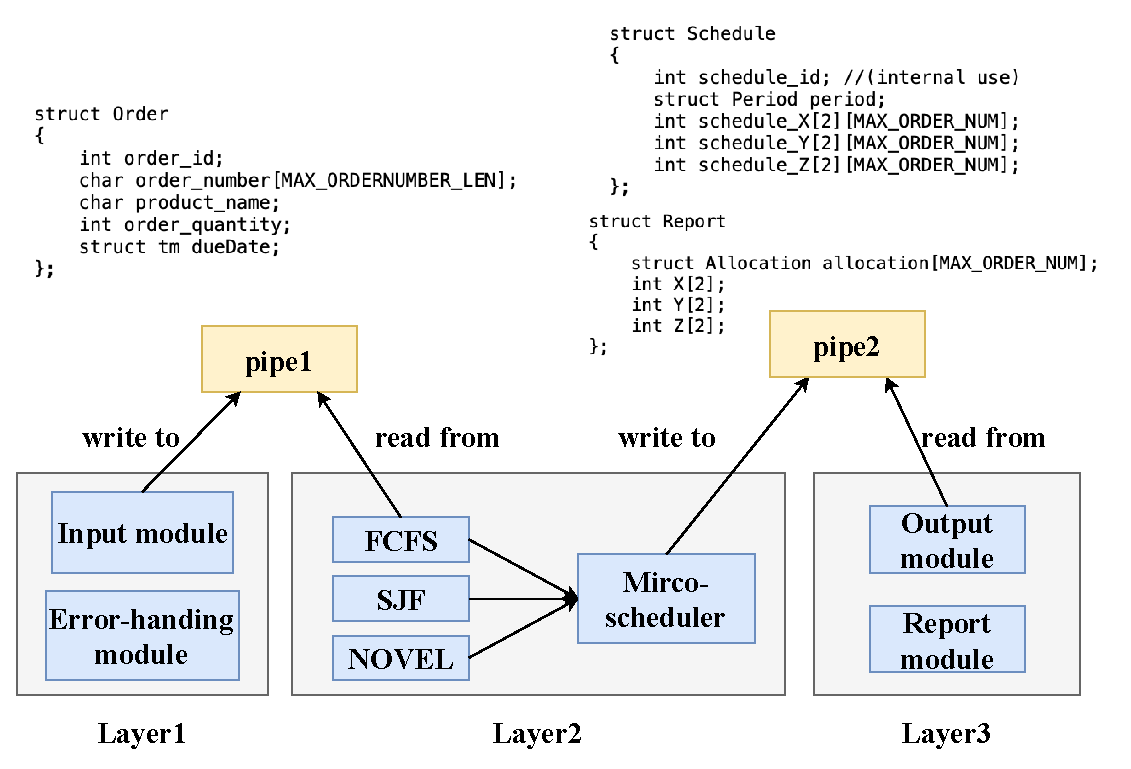
\includegraphics[width=0.9\columnwidth]{Figures/1.pdf}
\caption{Example of a full-column width figure.}
\label{fig:ex}
\end{figure}

\begin{itemize}
    \item \textbf{First Layer: } The first layer contains the Input module and error handling module, which will perform the UI and functionality as the requirement need: receive period, orders, batch of orders with due date checking and run the scheduler by using fork() system call that create a new process with respect to the required scheduling algorithm. The order list and period store in the data structure shared by the parent and child will the sent through an unnamed pipe. 
\end{itemize}

\begin{itemize}
    \item \textbf{Second Layer: } The second layer accommodates three scheduling algorithms and is the Scheduler module, which will receive order list and period from the p2c pipe, schedule the orders, and send back the schedule details Schedule and Report that is a shared data structure by child and parent through c2p pipe. The child process is the above-mentioned macro scheduler, and it will call another independent method called kernel which is the micro scheduler. Good  encapsulation is achieved since the responsibility of the micro scheduler is that dividing a number (order quantity) into 3 types of frames (daily capacity of three plants) with limited numbers of frames (the remaining days with respect to different plants before due date), thus, there is no dependency of micro scheduler onto macro scheduler.  Lastly, the schedule details are gathered in different forms: gathered by plants (sent via Schedule data structure) is for the Output module and gathered by orders (sent via Report data structure) is for Report module use.
\end{itemize}

\begin{itemize}
    \item \textbf{Third Layer: } The third layer is a relatively simpler tasks that in charge of the output and report format after decoding the data sent from layer two. 
\end{itemize}
And there is no need to consider the complexity of running different layers, we divide the layer concepts into actions with smaller granularity, and we believe this implementation is better for the Procedure Oriented Language like C. And the procedure transformation is shown is the figure.

\section{\textbf{Correctness Testing Cases}}
\subsection{Test Case Description}
The purpose of this test case is to validate the order processing capability of the Production Line Scheduler (PLS), ensuring it correctly handles order acceptance, rejection, and scheduling based on specified criteria such as due dates and production capacity.
\subsection{Test Order Batch File}
\begin{itemize}
    \item \textbf{Order 1:} \\
    \texttt{addORDER P0301 2024-06-02 1826 Product\_A} \\
    Expected to test the system's ability to reject orders that cannot be completed by the plant before the specified due date.
    \item \textbf{Order 2:} \\
    \texttt{addORDER P0302 2024-06-03 1330 Product\_B} \\
    Expected to test the system's capacity to accept orders and allocate resources within the permissible time frame.
    \item \textbf{Order 3:} \\
    \texttt{addORDER P0303 2024-06-04 1427 Product\_C} \\
    Aimed at testing the system's functionality to ignore orders that exceed the set due date.
\end{itemize}
\subsection{Processed Result}
\begin{itemize}
    \item \textbf{Order 1:} \\
    Product NO.0301 was rejected, as the production capabilities could not meet the tight deadline. This confirms the system's functionality in evaluating and rejecting unfeasible production requests based on current plant capacities and due dates.
    \item \textbf{Order 2:} \\
    Product NO.0302 was accepted, and the system scheduled two days for completion. This showcases the system's effective scheduling and resource allocation capabilities, ensuring that feasible orders are processed efficiently.
    \item \textbf{Order 3:} \\
    Product NO.0303 was ignored because it exceeded the due date of “2024-06-03”. This indicates the system's adherence to operational constraints and its ability to enforce order deadlines strictly.
\end{itemize}

\textbf{Output Screen: }
\begin{figure}[htbp]
\centering
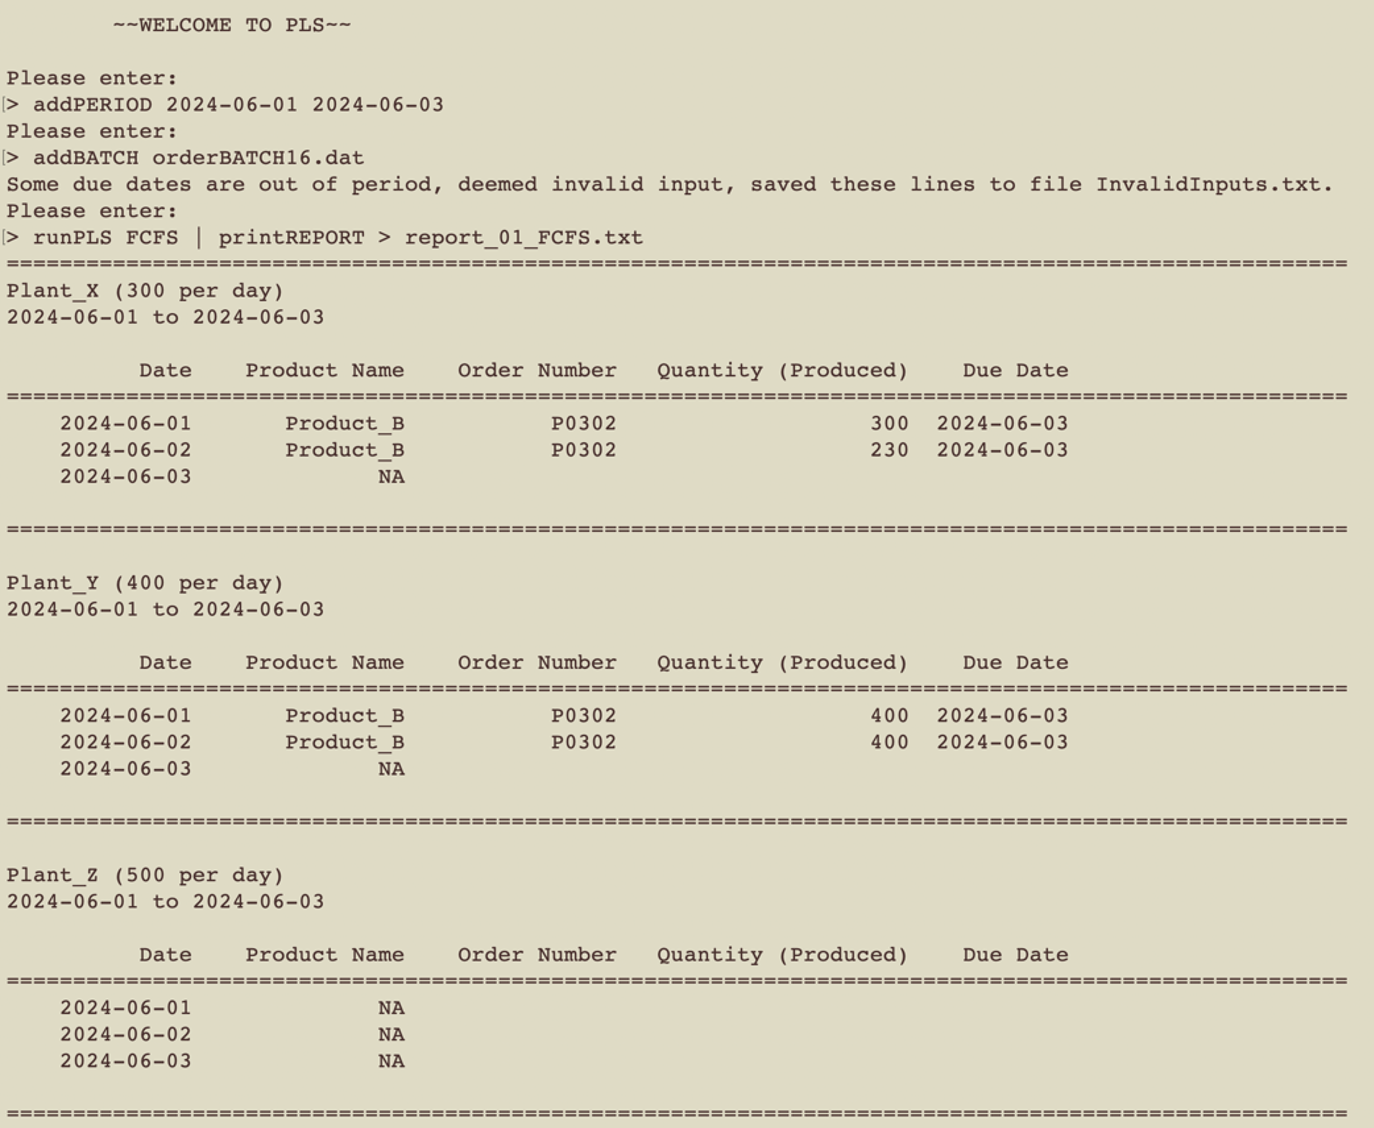
\includegraphics[width=0.9\columnwidth]{Figures/terminal.png}
\caption{This is the output on the terminal.}
\label{fig:terminal}
\end{figure}

\textbf{Report: }
\begin{figure}[htbp]
\centering
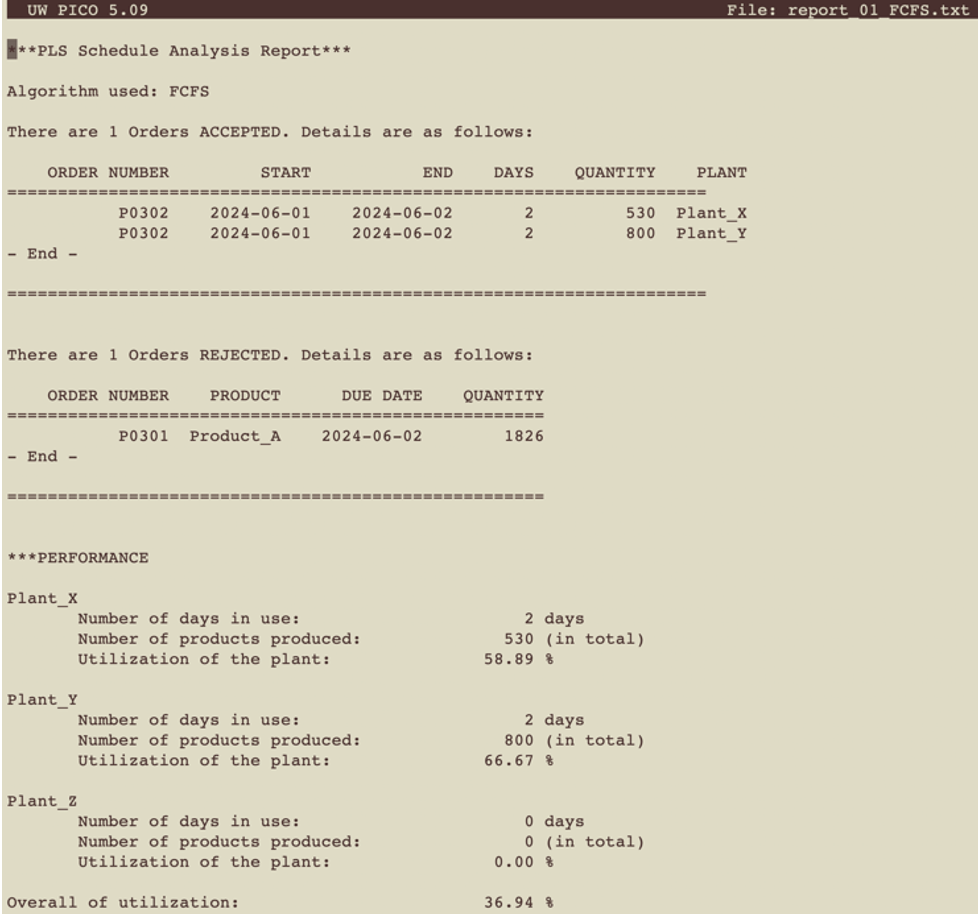
\includegraphics[width=0.9\columnwidth]{Figures/Report.png}
\caption{This is the report.}
\label{fig:Report}
\end{figure}

\subsection{Outcome Analysis}
The outcomes from the PLS align with the expected results, demonstrating the system's capabilities in:
\begin{itemize}
    \item \textbf{Adhering to Production Deadlines: } \\
    By rejecting orders that cannot be completed within the set deadlines, the system ensures operational efficiency and prevents overcommitment.
    \item \textbf{Resource Allocation: } \\
    Accepting and completing available orders within the designated timeframe shows effective resource management.
    \item \textbf{Enforcing Algorithm Rules: } \\
    Ignoring orders that exceed the due date highlights the system's strict compliance with algorithm policies.
\end{itemize}

\subsection{Conclusion}
These test orders confirm that the PLS operates correctly by adhering to algorithm rules. The system's ability to distinguish between feasible and infeasible orders, based on real-time data and predefined rules, ensures that production processes are both realistic and optimized. This testing phase not only validates the system's functional requirements but also reassures stakeholders of its reliability and efficiency in a live production environment.


\section{\textbf{Performance Analysis}}
We implement the micro scheduler for all three scheduling algorithms. Even through the micro scheduler is one of our innovative components tailored for the NOVEL scheduling, we apply it onto the other two algorithms to improve their utilization performances. It is reasonable because the naïve FCFS scheduling only consider the arrival sequence rather than the overall utilization. Therefore, we design the same efficient kernel for these three schedulers.
But still, the FCFS and SJF seldomly outperform NOVEL scheduling. As mentioned in last section, we believe that the utilization of assigning some relatively large orders then filled with smaller orders is better than assigning relatively small orders but leave large orders rejected. Therefore, the NOVEL algorithm is always better than the SJF scheduling as the running results show. While there is no relationship between the arrival sequence and quantity in our randomly generated data, so FCFS may be better than the NOVEL algorithm.

\section{\textbf{Program Set-up and Execution}}
This section provides detailed instructions on how to compile and execute the PLS (Product Line Scheduler) and discusses the Linux server environment used for testing and the results obtained.

\subsection{Compilation Instructions}
\begin{itemize}
    \item \textbf{Prerequisites:} \\
    Ensure you have the necessary development tools installed. For a C/C++ project, you might need gcc or g++, and be sure that they are installed on the computer or server.

    \item \textbf{Clone the Repository:} \\
    \begin{verbatim}
    git clone https://github.com/hi
    teacherIamhumble/PLS.git
    cd PLS
    \end{verbatim}

    \item \textbf{Compile the Project:} \\
    \begin{verbatim}
    gcc PLS.c -std=c99 -o PLS
    \end{verbatim}

    \item \textbf{Run the Application:} \\
    \begin{verbatim}
    ./PLS
    \end{verbatim}

    \item \textbf{See the Generated Files:} \\
    \begin{verbatim}
    pico orderBATCHXX.dat
    pico report_XX_XXXX.dat
    \end{verbatim}
\end{itemize}

\subsection{Library Required and Usage}
We include a series of libraries of C which provide the functionality of using pipes, creating and using child process, using time data structure and conveniently handling string data type.
In the below table, all the header files of our programs and the reasons they are used.

\begin{table}[htbp]
\centering
\caption{Special Libraries in Use to Support System}
\label{tab:my-table}
\resizebox{\columnwidth}{!}{%
\begin{tabular}{|c|l|}
\hline
\textbf{Library Used} & \multicolumn{1}{c|}{\textbf{Provided Functionality}} \\ \hline
\texttt{\textless stdlib.h\textgreater}            & Provide the exit() function to processes             \\ \hline
\texttt{\textless sys/stat.h\textgreater} &
  \begin{tabular}[c]{@{}l@{}}Provide the state of a child process back\\ to its parent process\end{tabular} \\ \hline
\texttt{\textless sys/wait.h\textgreater} &
  \begin{tabular}[c]{@{}l@{}}Provide waitpid() for a parent to ensure\\ a specific child ends successfully\end{tabular} \\ \hline
\texttt{\textless unistd.h\textgreater} &
  \multirow{2}{*}{\begin{tabular}[c]{@{}l@{}}Provide functions that create pipes,\\ close ends, and write/read from pipes.\end{tabular}} \\ \cline{1-1}
\texttt{\textless fcntl.h\textgreater}             &                                                      \\ \hline
\texttt{\textless string.h\textgreater}            & Provide strcmp() to handle string type               \\ \hline
\texttt{\textless time.h\textgreater} &
  \begin{tabular}[c]{@{}l@{}}Provide data structure tm to examine the \\ correctness of input date and calculate \\ the differences between two dates\end{tabular} \\ \hline
\end{tabular}%
}
\end{table}

\subsection{Linux Server Testing Environment}
We use the c99 rather than the default version of gcc compiler: c90.
Below is the basic information of the COMP appolo server that we run tests on.

\subsection{Test Results}
Test cases were executed to verify the scheduling and order handling capabilities of the PLS. The tests included scenarios like order acceptance, rejection based on capacity, and deadline adherence.

\begin{figure}[htbp]
\centering
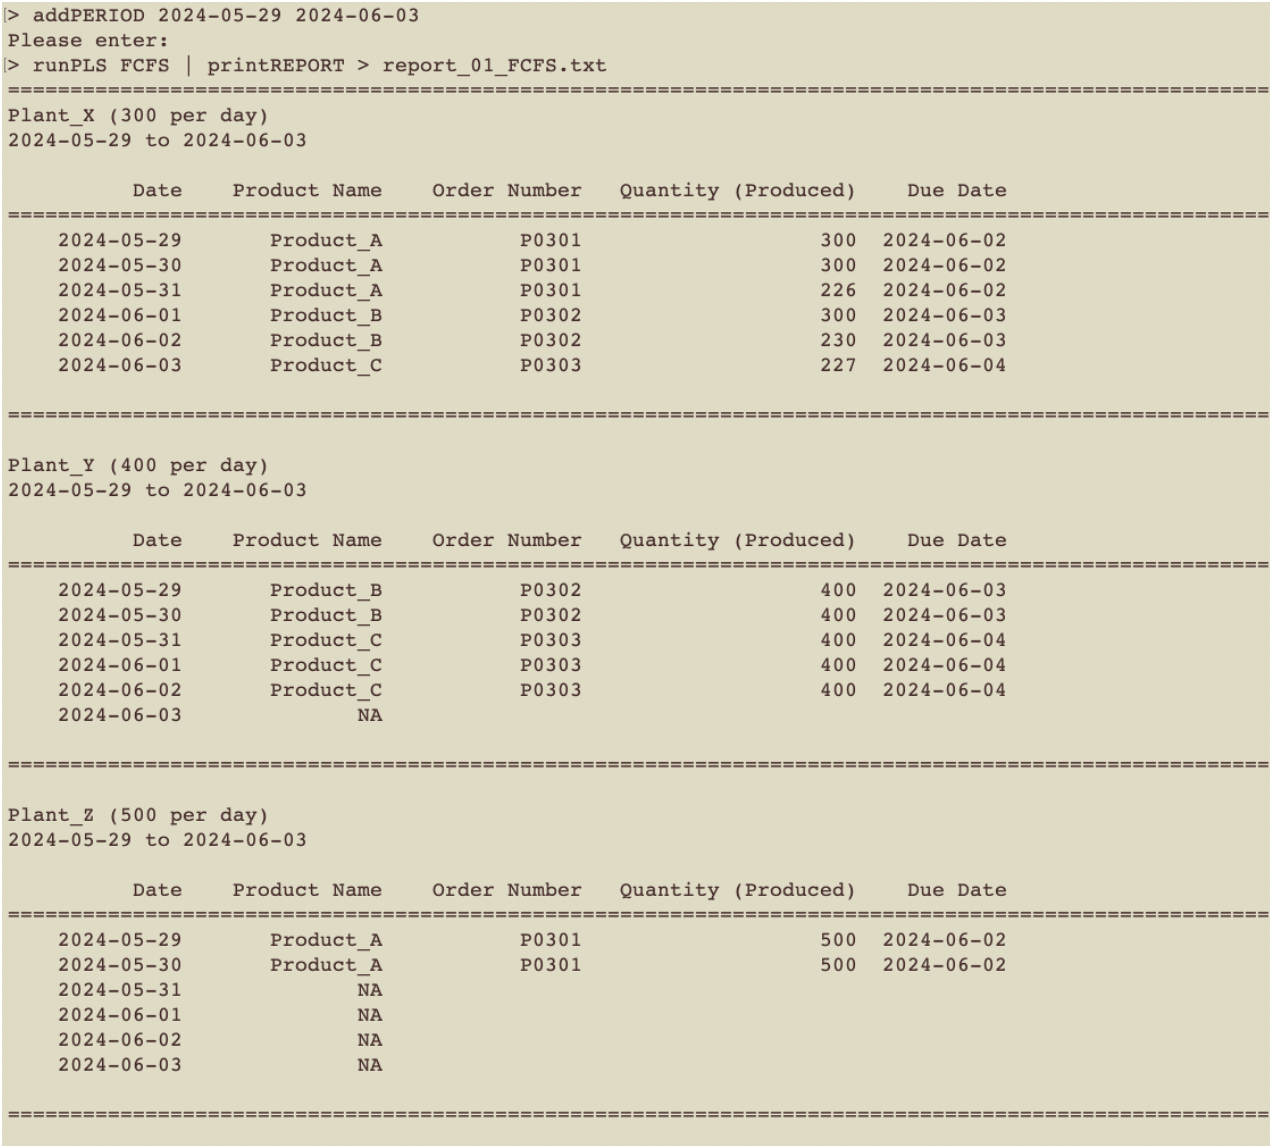
\includegraphics[width=0.9\columnwidth]{Figures/Output.png}
\caption{This is the output on the terminal}
\label{fig:Output}
\end{figure}

\subsection{Conclusion}
All test cases passed successfully. The scheduler was able to handle multiple concurrent orders and optimize the production line efficiently


\section{\textbf{Result Discussion}}
We generate 5 random order batches by Microsoft excel and test them on the three scheduling algorithms. And the results are shown in the following table:

\begin{table}[htbp]
\centering
\caption{Performance Results}
\label{tab:mm}
\resizebox{0.8\columnwidth}{!}{%
\begin{tabular}{|l|l|l|l|}
\hline
Batch no. & FCFS    & SJF     & NOVEL   \\ \hline
1         & 62.49\% & 60.52\% & 69.69\% \\ \hline
2         & 76.95\% & 71.24\% & 76.95\% \\ \hline
3         & 78.25\% & 81.73\% & 85.77\% \\ \hline
4         & 59.43\% & 59.43\% & 59.43\% \\ \hline
5         & 55.99\% & 55.99\% & 61.71\% \\ \hline
\end{tabular}%
}
\end{table}

The table provides utilization percentages for different batches processed through three scheduling algorithms: First-Come First-Served (FCFS), Shortest Job First (SJF), and our NOVEL algorithm (NOVEL). Upon analysis, it's evident that the NOVEL algorithm consistently outperforms FCFS and SJF in terms of plant utilization across all batches.
In Batch 1, NOVEL achieves a utilization rate of 69.69\%, surpassing FCFS (62.49\%) and SJF (60.52\%). This trend continues in Batch 2 and Batch 3, where NOVEL maintains or exceeds the highest utilization percentages among the three algorithms. Particularly noteworthy is Batch 3, where NOVEL achieves an impressive 85.77\% utilization rate compared to FCFS (78.25\%) and SJF (81.73\%).
The superior performance of NOVEL can be attributed to its unique prioritization of orders based on larger quantities. By favoring high-volume orders, NOVEL optimizes throughput and resource allocation, thereby maximizing plant utilization. This is evident in the consistently higher utilization rates observed across all batches.
Furthermore, the NOVEL algorithm demonstrates resilience in Batch 4, where all algorithms yield identical utilization rates (59.43\%). While FCFS and SJF falter in adapting to the batch's characteristics, NOVEL maintains its effectiveness by efficiently handling orders with larger quantities.
In Batch 5, NOVEL continues to exhibit its superiority, achieving a utilization rate of 61.71\% compared to FCFS and SJF, both at 55.99\%. This further reinforces the efficacy of the NOVEL algorithm in dynamically managing production schedules and optimizing resource utilization.
Overall, the results highlight the significant advantages of the NOVEL algorithm in enhancing plant utilization and optimizing production schedules in a real-world manufacturing context. Its ability to adapt to varying batch characteristics and prioritize high-volume orders underscores its potential for driving efficiency and productivity in industrial settings.


\section{\textbf{Conclusion}}
In this steel-making plant problem, we made great efforts to solve the scheduling inefficiencies. By incorporating CPU scheduling algorithm ideas into the structure of our production line scheduler (PLS), we've accomplished better resource allocation and overall system performance. Through development and implementation of our program in a Linux environment, we've created a dynamic platform which is capable of adjusting to real-time needs and requirements. This versatility means that our scheduler can respond to changing production demands, reducing delays, and increasing throughput across numerous sites. 

Besides, the use of traditional CPU scheduling methods such as First-Come First-Served (FCFS) and Shortest Job First (SJF), combined with our new strategy that prioritizes greater volumes, has provided significant inspirations of the intricacies of production scheduling. We investigated how each algorithm operates under different settings, which reveals their relative strengths and drawbacks in the industrial environment. Furthermore, our project components' structural was close to essential operating system features, such as work queues and system monitoring tools, and it allows for the combination of theoretical concepts and practical applications. This consistency not only accelerates the development process, but also establishes a conceptual framework for future improvements and revisions.

In conclusion, our performance analysis has revealed actionable knowledge for the medium-size steel-making manufacturer, allowing him to make more smart decisions and prepare strategically. The manufacturer may use the data supplied by our scheduler to improve their operations, eliminate idle time, and eventually become more competitive in the industry. In essence, our project applies computer science insights to real-world manufacturing difficulties. As we continue to improve and extend our scheduling, we are dedicated to fostering innovation and efficiency in the ever-changing face of industrial production. 

\section{\textbf{References}}
\bibliographystyle{plain}
\bibliography{ref}

\section{\textbf{Innovative Scheduling Algorithm: NOVEL}}
\textbf{Since the FCFS and SJF Scheduling algorithms mainly take consideration on the arrival sequence and quantity number rather than the overall utilization of the three plants, which is the only judgement on PLS task, our group aims to design an innovative algorithm to reach better utilization. The design details, considerations and analysis are discussed in this section.}
\subsection{\textbf{Analysis on brute-force algorithm}}
\textbf{It is not difficult to find brute-force algorithm always generate the schedule with best utilization by comparing each possible schedules. However, it is not recommended for its time complexity and naïve idea without innovation. Even though some improvements could be made during comparation, the time complexity still requires O(2n * 3n * n!) for n orders in the worst case. In addition, because of its lack of analysis on the real problems, this scheduling suffers from its lack of creativity. Therefore, we recommend an algorithm using greedy idea and a series of improvements out of real needs.}
\subsection{\textbf{Reanalysis on PLS task}}
\textbf{Before going into details of our algorithm, a deeper look onto the PLS task is recommended, where you could discover the design considerations. 
For one, we regard a schedule as two components that is fragment and production, based on the states of the three plants idle and active. Therefore, to improve the overall utilization given by a specific period only needs to decrease the number of fragments. Take a closer look into the fragments, we divided them into two types: internal fragments and external fragments. Internal fragments refer to the idle state of a plant for one day, which is cause by the assigned production quantity is less than the capacity of the plant of one day. While the external fragments mean the whole idle state of one day with respect to a factory, which is caused by rejected orders could not be finished by that plant before order due date. In our design, we aim to lower both internal fragments and external fragments.
For another, we focus on the numerator and denominator of the utilization formula. The denominator of utilization is unchanged when comparing different algorithms based on the same order set and production period. While the numerator is indeed the total sum of accepted orders. In this point of view, utilization improvement under same input (orders and period) is nothing but accept as many as possible orders.}
\subsection{\textbf{Design and Implementation Details}}
\textbf{On the one hand, fragmentations are decreased by using a combination of greedy and brute-force idea. More precisely, we design a macro scheduler aiming to lower external fragments and a micro scheduler which makes sure reach the least internal fragments. After given all the orders, the macro scheduler will sort the orders again in a descending quantity order then do the same thing as FCFS. This is reasonable to decrease external fragmentations because we believe the utilization of assigning some relatively large orders then filled with smaller orders is better than assigning relatively small orders but leave large orders rejected. Though this assumption may make mistakes under specific order batch, we design a performance test over randomly generated order quantity and due date, which proves this scheduling outperforms than FCFS and SJF. In addition, the macro scheduler decides the decline of orders, which is that the scheduler will exam if the current waiting order could be finished by three plants before its due days. We won’t reject orders if they could be done without reserving space for the coming orders because we want to make sure every order assignment will perform best under current condition. This is also the drawback of the greedy idea that couldn’t promise the optimal scheduling. After deciding the accepted order, the macro scheduler will ask the micro scheduler to decide how to allocate on three plants. At last, the macro scheduler will update the plant states based on the micro scheduler and move to the next order.
On the other hand, the micro scheduler is given the remaining days of X, Y, Z plants before due date and total quantity the order requires. The micro scheduler will use brute-force design to compare all the distribution and decide the optimal one with least internal fragmentations. Then the allocation details will be sent back to the macro scheduler. At this point, the external and internal fragmentations is reduced in an optimized way.
Last but not least, as we try to accept as many as orders as we could, we redesign the enumerate sequence and comparation conditions inside the micro scheduler and make sure if there are multiple schedule of the same least internal fragmentations, the final allocation will first use the plant X to remaining plant Z with larger daily capacity for accommodating more future orders. The pseudocode of the macro and micro scheduler is shown below for efficient understanding.}

\begin{algorithm}
\renewcommand{\thealgorithm}{1} % This sets the algorithm number
\caption{Macro Scheduler of NOVEL} % Caption for the algorithm
\begin{algorithmic}[1] % The [1] option enables line numbering
    \State \textbf{reorder} the orders in a descending quantity order
    \For{\textbf{each} order in order\_set}
        \State Calculate the remain days of X, Y, Z plants before due
        \State Calculate the capacity
        \If{\(capacity < Q\)}
            \State reject the order
            \State \textbf{break}
        \EndIf
        \State \(\textbf{micro\_scheduler}(X\_rem, Y\_rem, Z\_rem, Q)\)
        \State update the X, Y, Z plants states
    \EndFor
\end{algorithmic}
\end{algorithm}

\begin{algorithm}
\caption{Micro Scheduler Function}
\begin{algorithmic}[1] % Enables line numbering
\Function{micro\_scheduler}{$X\_rem, Y\_rem, Z\_rem, Q$}
    \State $vac \gets Q$
    \State $x \gets 0$
    \State $y \gets 0$
    \State $z \gets 0$
    \For{$i \gets 0$ \textbf{to} $\lfloor Q/300 \rfloor$}
        \For{$j \gets 0$ \textbf{to} $\lfloor Q/400 \rfloor$}
            \For{$k \gets 0$ \textbf{to} $\lfloor Q/500 \rfloor$}
                \State $rem \gets Q - 300 \cdot i - 400 \cdot j - 500 \cdot k$
                \If{$rem \geq 0$ \textbf{and} $rem \leq vac$}
                    \State $x \gets i$
                    \State $y \gets j$
                    \State $z \gets k$
                    \State $vac \gets rem$
                \EndIf
            \EndFor
        \EndFor
    \EndFor
    \State \Return $\{x, y, z, vac\}$
\EndFunction
\end{algorithmic}
\end{algorithm}

\subsection{\textbf{Deficiency and Improvements}}
\textbf{Since greedy algorithm is applied, the NOVEL algorithm cannot promise to produce the optimal schedule, or even worse, produce the schedule worse than FCFS or SJF. Therefore, a checking mechanism is introduced in macro scheduler, which will compare the schedule with other two scheduling algorithms before sending back to other modules in pipe(). The final schedule with the best overall utilization will be sent back to enhance performance. The performance experiments in Section eight provides a more straightforward optimization on NOVEL algorithm over the other two scheduling.
}

\section{\textbf{Appendix}}

\subsection{Source Code}
\lstinputlisting[language=C, caption=PLS Source Code]{Figures/PLS_G20.c}

\subsection{Sample Outputs}

\begin{figure}[htbp]
\centering
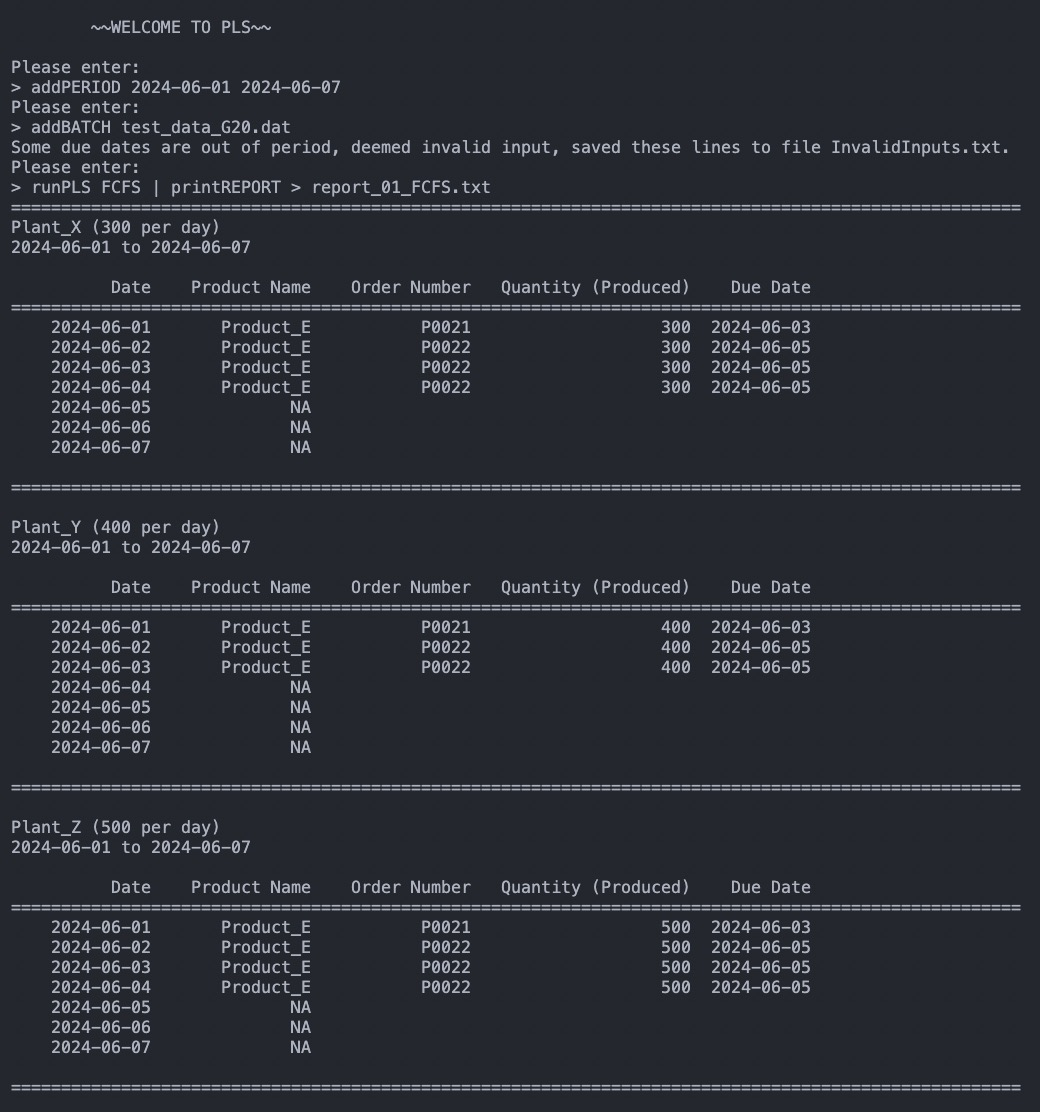
\includegraphics[width=0.6\columnwidth]{Figures/1.jpg}
\caption{This is the output on the terminal of FCFS algorithm.}
\label{fig:FCFS}
\end{figure}
\end{document}
